\documentclass[aspectratio=169]{beamer}
\usetheme{Madrid}
\usepackage[utf8]{inputenc}
\usepackage[T1]{fontenc}
\usepackage{tikz}
\usepackage{amssymb}
\usepackage{graphicx}
\setbeamertemplate{navigation symbols}{}
\setbeamercolor{title}{fg=white,bg=magenta!70!red}
\setbeamercolor{frametitle}{fg=white,bg=magenta!70!red}
\setbeamercolor{block title}{bg=magenta!70!red!20,fg=black}
\setbeamercolor{block body}{bg=magenta!70!red!8,fg=black}
\setbeamercolor{item}{fg=magenta!70!red}
\setbeamercolor{itemize item}{fg=magenta!70!red}
\setbeamertemplate{itemize item}[triangle]

\title{Foundations 3 — Your First Code}
\subtitle{Variables, text vs. numbers, arithmetic --- starting from absolute zero}
\author{ByteForge --- Grade 9 --- The Deep Diver}
\date{}

\begin{document}

\begin{frame}
    \titlepage
\end{frame}

\begin{frame}{Today's Missions}
    \Large
    \begin{itemize}
        \item Learn: What Is a Variable?
        \item Store a Number
        \item What Kind of Value?
        \item Do the Math
        \item Combine Two Texts
    \end{itemize}
\end{frame}

\begin{frame}{A variable is a labelled box, nothing more}
    \large
    \begin{itemize}
        \item It stores ONE value so your code can use it again later
        \item \texttt{score = 10} --- the = means "store this", NOT "equals" like in maths
        \item Whatever was in the box before gets completely overwritten
    \end{itemize}
\end{frame}


\begin{frame}{Quotes are the entire difference between text and number}
    \large
    \begin{itemize}
        \item \texttt{10} --- a real number (an integer), you can do maths with it
        \item \texttt{"10"} --- text (a string) that just LOOKS like a number --- no quotes, no maths
        \item Mixing these two up is the single most common real beginner mistake
    \end{itemize}
\end{frame}


\begin{frame}{+ means something different for numbers vs. text}
    \large
    \begin{itemize}
        \item Numbers: \texttt{4 + 7} genuinely adds --- gives you \texttt{11}
        \item Text: \texttt{"Systems " + "Online"} STICKS them together --- gives you \texttt{"Systems Online"}
        \item Same symbol, completely different job, depending on the type
    \end{itemize}
\end{frame}

\begin{frame}{Real-World Examples}
    \large
    \begin{itemize}
        \item A game's health value (100, then 75, then 50) is a real variable, changing exactly like \texttt{score = 10} then \texttt{score = 20}.
        \item A username field that will not accept a number as your name is enforcing exactly this "quotes = text" distinction.
    \end{itemize}
\end{frame}


\begin{frame}{Image}
    \begin{center}
    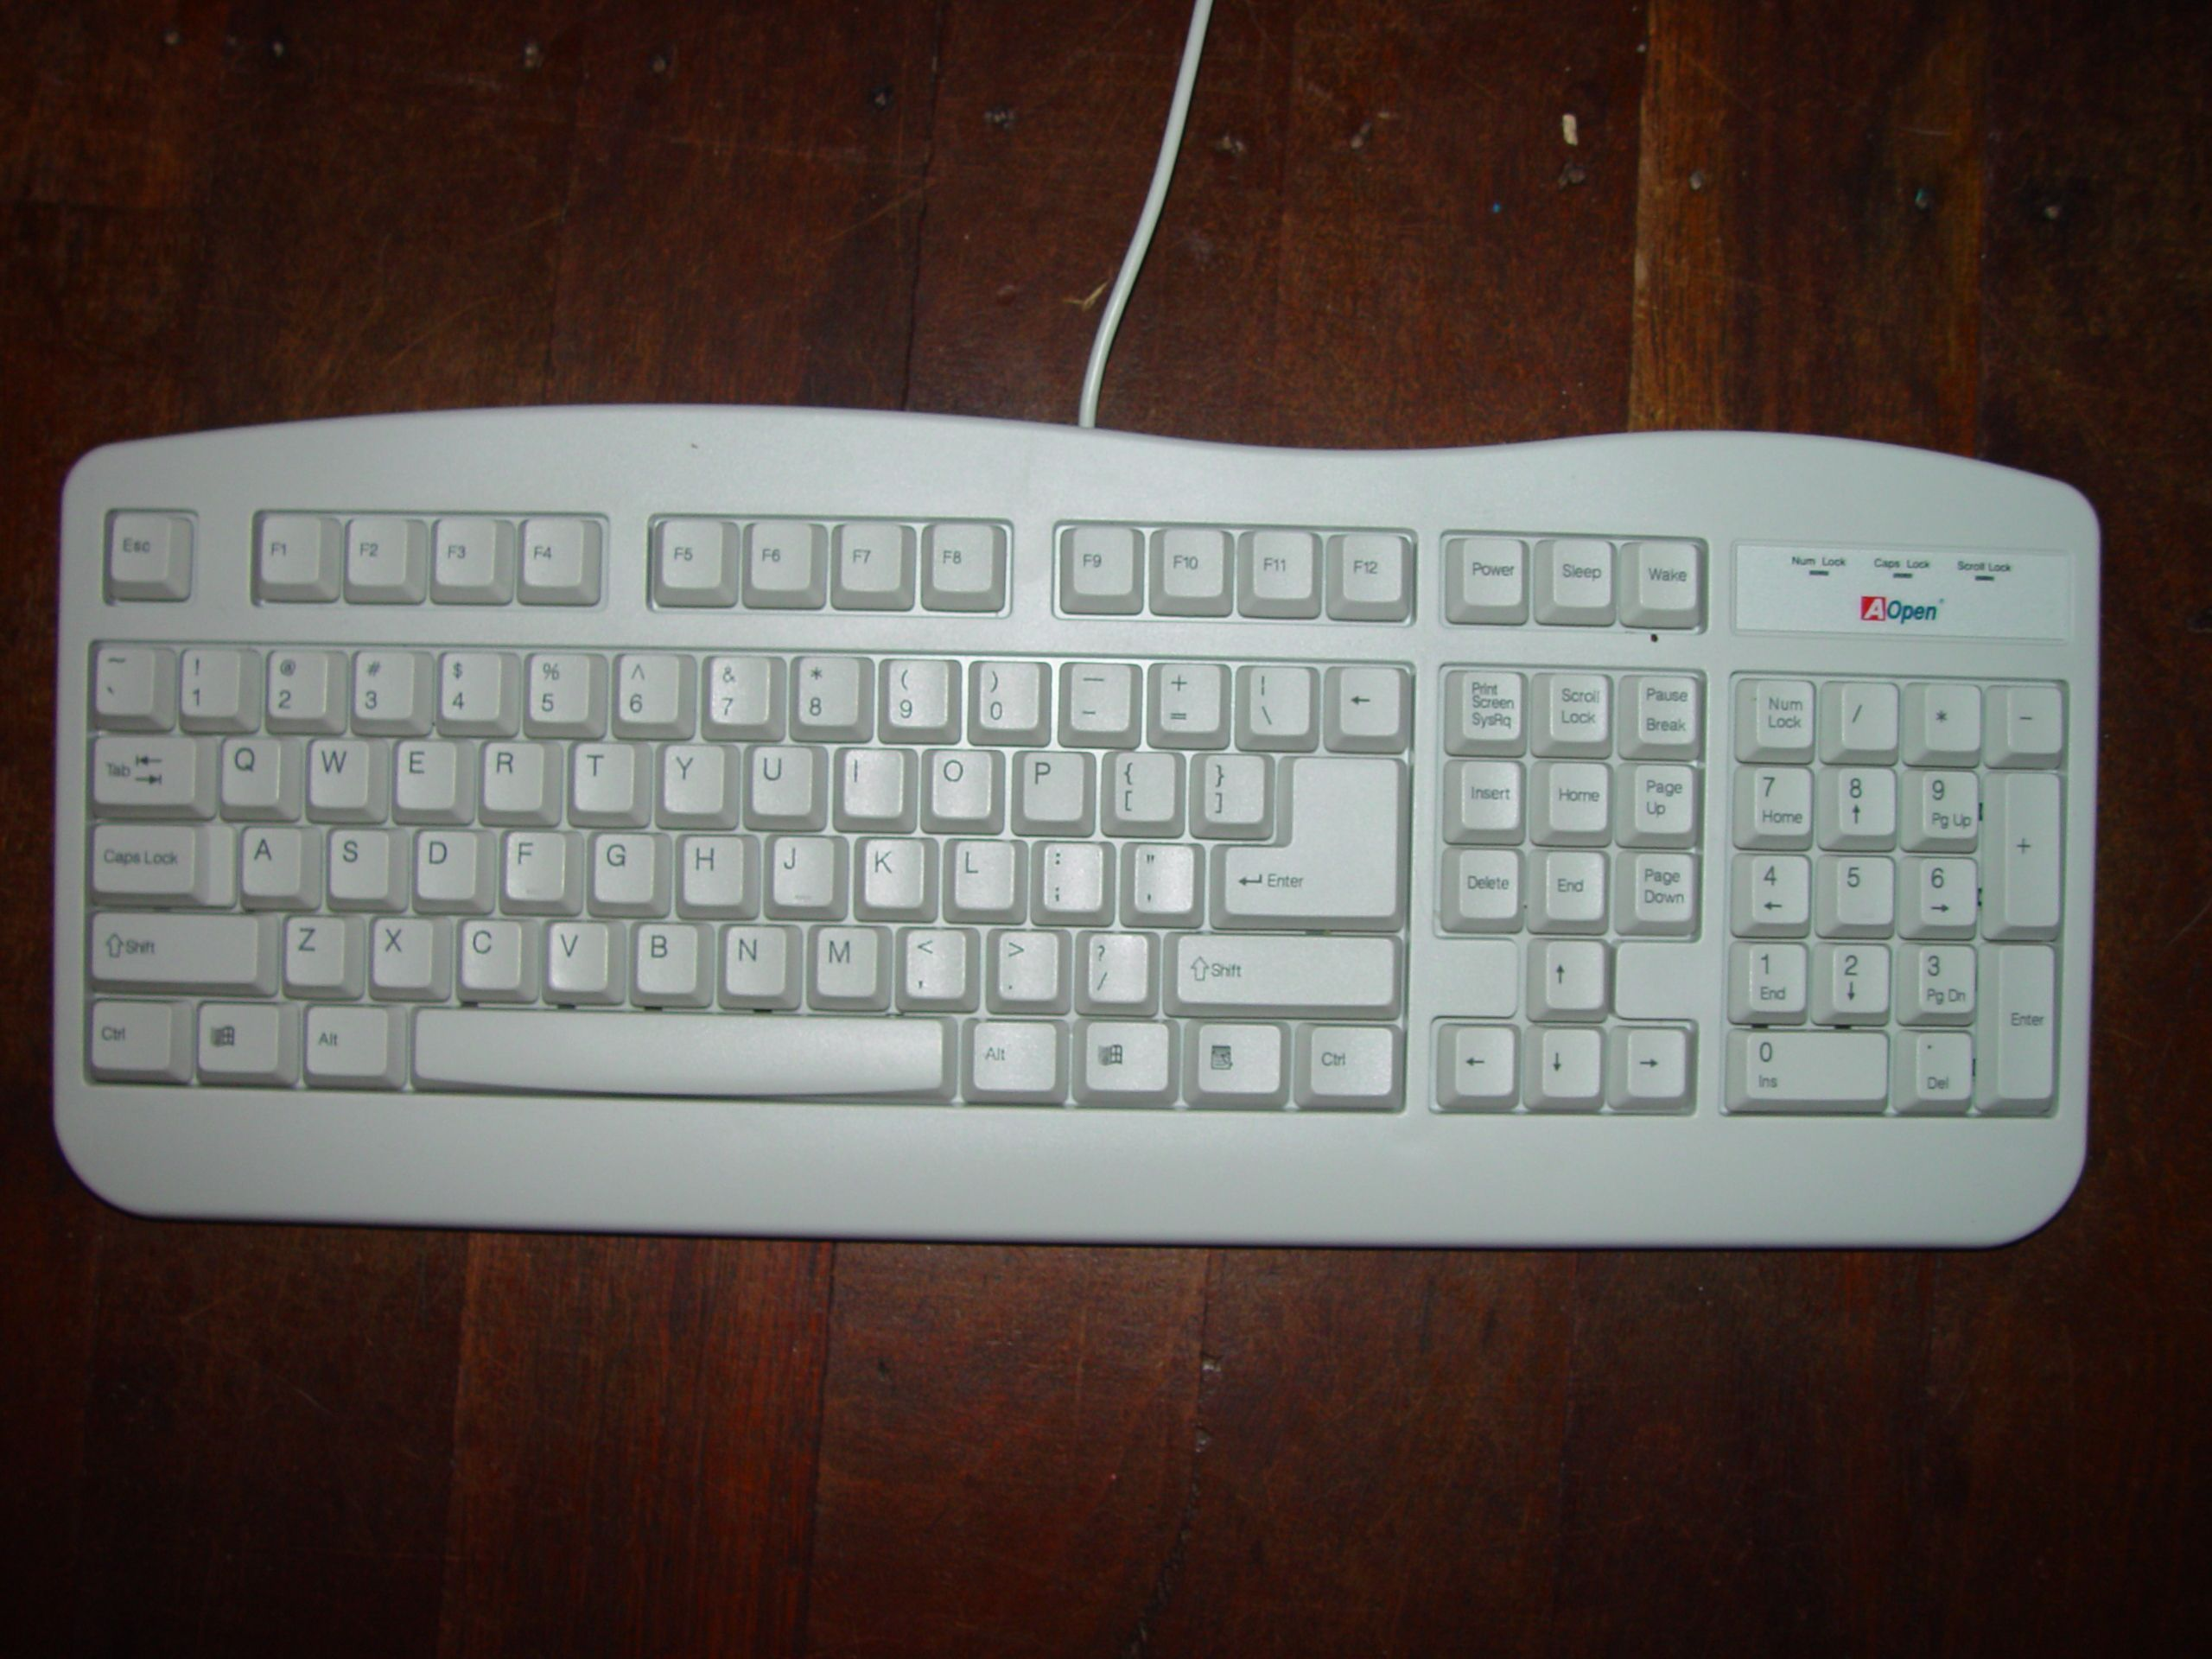
\includegraphics[width=0.5\textwidth]{images/keyboard.jpg}

    \large Every single line of real code you are about to write starts by typing on a keyboard exactly like this one.

    \small Computer keyboard, public domain, via Wikimedia Commons
    \end{center}
\end{frame}

\begin{frame}{Let Them Discover}
    \large
    Before opening the platform: on paper, write down 3 real variables a video game needs to track (score, lives, time). For each one, is it a NUMBER or TEXT?
\end{frame}

\begin{frame}{Your Turn}
    \Large
    Open the mission map, find \textbf{Foundations 3 — Your First Code}, and fly it for real ---
    everything you just saw, you now do yourself.
\end{frame}

\end{document}
